% Source code of the TAutoCorr.R results interpretation
% Author: Shuqing Ren (sr1822@ic.ac.uk)
% Question: Are temperatures of one year significantly correlated with 
% the next year (successive years), across years in a given location?

\documentclass[12pt, a4paper]{article}
\usepackage{graphicx} 
\usepackage[margin=2cm]{geometry} 

\title{Autocorrelation in Florida weather}

\begin{document}
  \maketitle

  % discriptive stats (include or delete???)
  Data of Florida annual mean temperaturs were collected for a centry (100 years) 
  between 1901 and 2000. The annual mean temperatures ranges from 23.75 to 
  26.35 degree Celsius, with a mean of 25.31 (SD = 0.50).

  % correlation coefficient & apparent asymptotic p-value
  The Pearson correlation coefficient of annual mean temperatures between 
  successive year pairs was ???, showing a ??? autocorrelation.
  As figure \ref{fig:plot} shows, an annual mean temperature is likely to increase 
  as that of its previous year increases. The correlation was statistically ??? 
  with an approximate p-value ???, calculated from permutation analysis (simulation time = ???).

  % figure
  \begin{figure}[h]
    \centering
    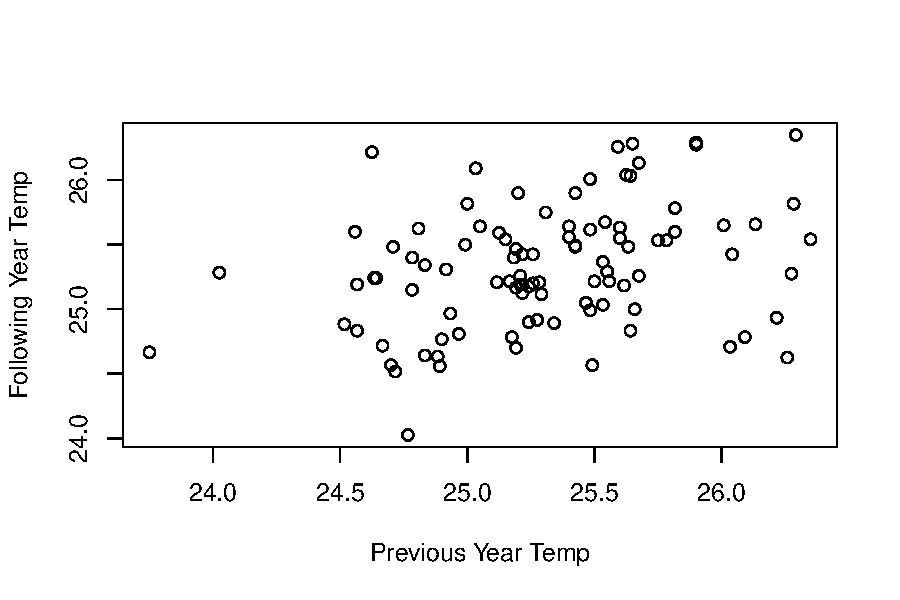
\includegraphics[width=0.9\textwidth]{../results/Fig1.pdf}
    \caption{Autocorrelation of succesive years in Florida weather. 
    Each point represents the mean tempreture (Temp) of a year responding to 
    the mean tempreture of its previous year.}
    \label{fig:plot}
  \end{figure}

\end{document}